\documentclass{article}

% Language setting
% Replace `english' with e.g. `spanish' to change the document language
\usepackage[english]{babel}

% Set page size and margins
% Replace `letterpaper' with `a4paper' for UK/EU standard size
\usepackage[a4paper,top=2cm,bottom=2cm,left=3cm,right=3cm,marginparwidth=1.75cm]{geometry}

% Useful packages
\usepackage{amsmath}
\DeclareMathOperator{\sinc}{sinc}

\usepackage{amssymb}

\usepackage{graphicx}
\usepackage[colorlinks=true, allcolors=blue]{hyperref}


\usepackage{tikz}
\usetikzlibrary{arrows,decorations.pathmorphing,backgrounds,fit,positioning,shapes.symbols,chains,shapes.geometric,shapes.arrows,calc}


\usepackage{listings}
\usepackage{xcolor}
\usepackage{enumitem}
\usepackage{physics}
\usepackage{float}
\setlist[itemize]{nosep} 

% custom code formatting with lstlisting
\definecolor{codegreen}{rgb}{0,0.6,0}
\definecolor{codegray}{rgb}{0.5,0.5,0.5}
\definecolor{codepurple}{rgb}{0.58,0,0.82}
\definecolor{backcolour}{rgb}{0.95,0.95,0.92}

\lstdefinestyle{mystyle}{
    backgroundcolor=\color{backcolour},   
    commentstyle=\color{codegreen},
    keywordstyle=\color{magenta},
    numberstyle=\tiny\color{codegray},
    stringstyle=\color{codepurple},
    basicstyle=\ttfamily\footnotesize,
    breakatwhitespace=false,         
    breaklines=true,                 
    captionpos=b,                    
    keepspaces=true,                 
    numbers=left,                    
    numbersep=5pt,                  
    showspaces=false,                
    showstringspaces=false,
    showtabs=false,                  
    tabsize=2
}

\lstset{style=mystyle}

% remove the paragraph indentation
\setlength{\parindent}{0pt}

\title{Homework 2, Reti Di Calcolatori}
\author{Matteo Galiazzo}

\begin{document}
\maketitle

\tableofcontents

\section{Come eseguire il codice}

Il codice è stato sviluppato su \verb|macos 14.4.1| e \verb|Ubuntu 23.10|.

Per eseguire il codice bisogna avere \verb|python3| (il codice è stato testato su \verb|Python 3.12.3| e \verb|Python 3.11.6|) e le librerie:
\begin{itemize}
  \item ping3
  \item numpy
  \item pandas
  \item matplotlib
\end{itemize}

\textbf{Per eseguire la parte di codice che esegue i ping con ping3 potrebbe essere necessario avere i privilegi da amministratore (sudo)}

Per eseguire il codice basta digitare il seguente comando dalla directory principale del progetto:

\begin{lstlisting}
python3 main.py
\end{lstlisting}

\section{Parametri dell'esperimento}

Per l'esperimento sono stati scelti i seguenti parametri:
\begin{itemize}
  \item \textbf{server}: \verb|paris.testdebit.info|
  \item \textbf{numero di istanze $k$}: \verb|100|
  \item \textbf{dimensione dei pacchetti}: la dimensione dei pacchetti è stata generata usando la funzione \verb|np.linspace(10, 1472, 75, dtype = int)|, e contiene quindi 75 dimensioni diverse a intervalli regolari che variano tra 10 e 1472.
\end{itemize}

\section{Stima del numero di link attraversati}

Sono stati attraversati 16 link usando il comando \verb|traceroute|, e lo stesso numero è stato stimato usando il comando \verb|ping| e variando il suo TTL.

\section{Andamento dell'RTT in funzione della dimensione del pacchetto}

\begin{figure}[H]
  \centering
  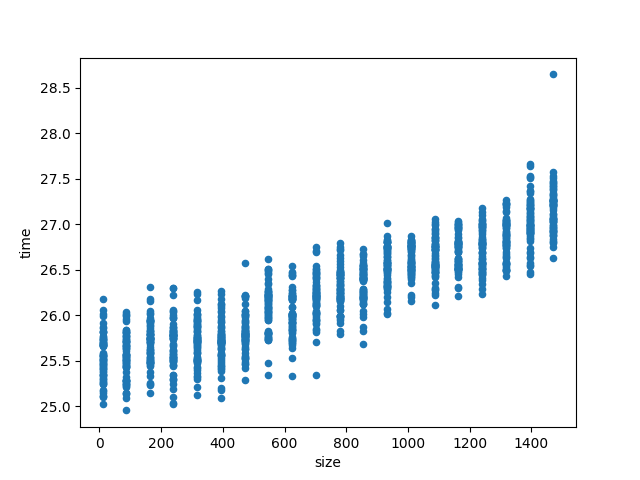
\includegraphics[width=0.45\linewidth]{rtt_data.png}
  \caption{RTT in funzione della dimensione del pacchetto}
  \label{fig:rtt_data}
\end{figure}

\subsection{RTT minimo}

\begin{figure}[H]
  \centering
  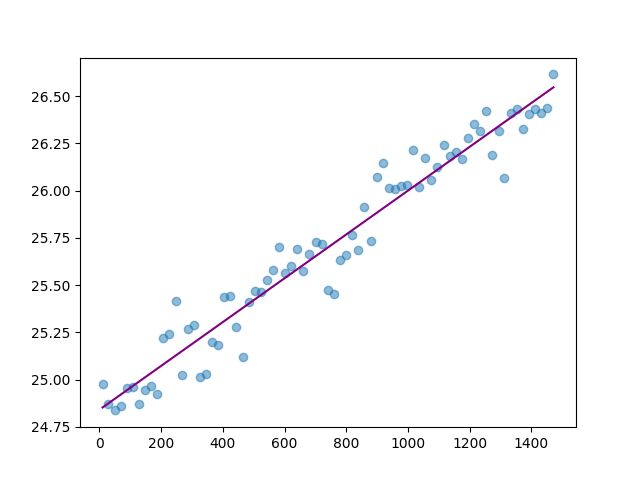
\includegraphics[width=0.45\linewidth]{rtt_min_fit.png}
  \caption{RTT minimo in funzione della dimensione del pacchetto}
  \label{fig:rtt_min_data}
\end{figure}

Il fit è la retta $y = 1.16 * 10^{-3} x + 2.48$

\subsection{RTT medio}

\begin{figure}[H]
  \centering
  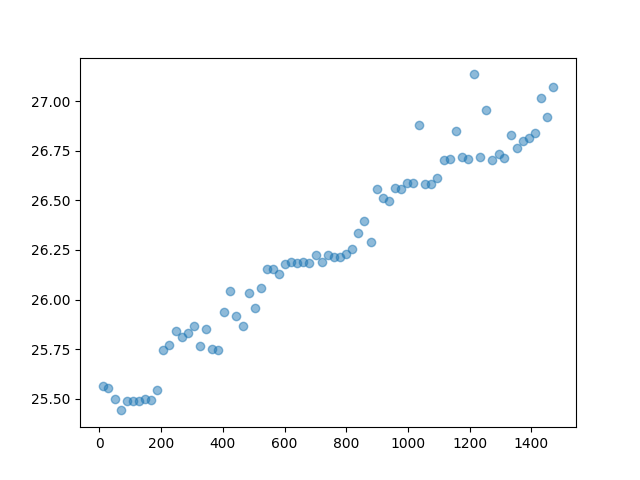
\includegraphics[width=0.45\linewidth]{rtt_avg_data.png}
  \caption{RTT medio in funzione della dimensione del pacchetto}
  \label{fig:rtt_avg_data}
\end{figure}

\subsection{RTT massimo}

\begin{figure}[H]
  \centering
  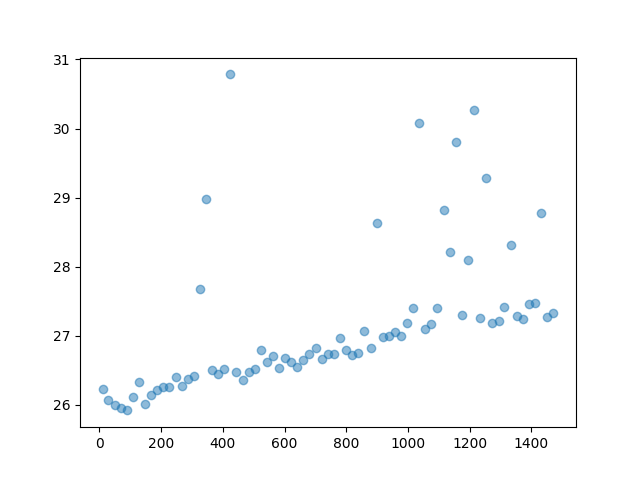
\includegraphics[width=0.45\linewidth]{rtt_max_data.png}
  \caption{RTT massimo in funzione della dimensione del pacchetto}
  \label{fig:rtt_max_data}
\end{figure}

\subsection{Deviazione standard del RTT}

\begin{figure}[H]
  \centering
  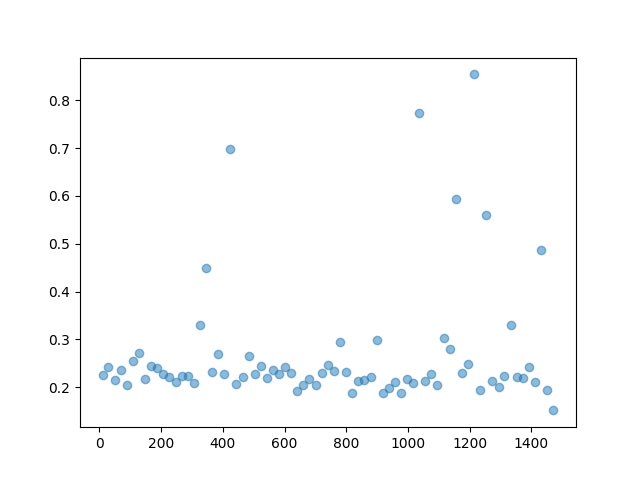
\includegraphics[width=0.45\linewidth]{rtt_stddev_data.png}
  \caption{Deviazione standard del RTT in funzione della dimensione del pacchetto}
  \label{fig:rtt_stddev_data}
\end{figure}

\section{Stima di $R$ e $R_{bottleneck}$}

\section{Discussione dei risultati ottenuti}

\end{document}